\documentclass[12pt,fleqn]{article}\usepackage{../../common}
\begin{document}
Materyel Mekaniği - 5

Bükülen bir çubuğun formüllerine bir giriş [1] kaynağında yapıldı. Orada
moment-eğri (moment-curvature) formülü gösterilmişti.

$$
M(x) = \frac{E(x)I(x)}{\rho(x)}
\mlabel{1}
$$

Şimdi bu formülü genişletelim, ve bir ikinci derece türeve eşitleyelim.

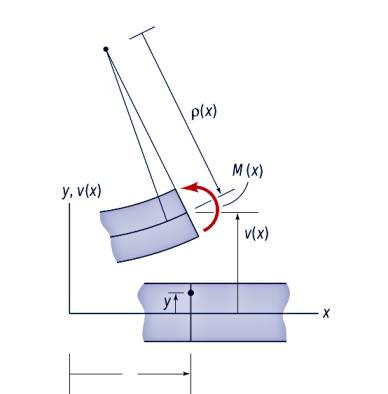
\includegraphics[width=15em]{phy_020_strs_05_01.jpg}

Resimde gösterilen semboller $M$ bükme momenti, $\rho$ çubuğun $+y$ tarafındaki
bükülme çemberinin, eğiminin yarıçapı (radius of curvature).  $v$ ise yine $+y$
kısmındaki yer değişimidir. Çubuğa uygulanan kuvvet dağılımının ne olduğu
önemli değil, sonuçta odaklandığımız çubuğun ufak bir kısmı.

[3] kaynağında bir çemberi (yarıçapını) onun bir eğriye dokunduğu noktadaki
türevler üzerinden temsil etme tekniğini paylaştık. Bu formülü mevcut probleme
uygulayabiliriz.

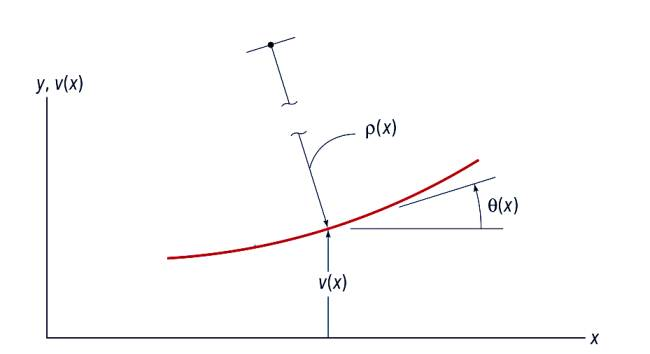
\includegraphics[width=20em]{phy_020_strs_05_02.jpg}

Üstteki örnekte çemberin yarıçapı $\rho$, türevler ise $\ud v / \ud x$.
Formül [2, sf. 466],

$$
\frac{1}{\rho} =
\frac
{\dfrac{\ud^2 v}{\ud x^2}}
{ \left[ 1 + \left( \dfrac{\ud v}{\ud x}  \right)^2 \right]^{3/2} }
$$

Üstteki problemde eğim çok ufaktır o zaman $\ud v / \ud x$ ufak kabul edilir
(resimdeki eğim eğitim amaçlı abartılmış), demek ki bölendeki kare hesabı
daha da ufalır, geriye sadece 1 kalır, 1 ile bölümü yok sayarız, geriye kalanlar

$$
\frac{1}{\rho} \approx \frac{\ud^2 v}{\ud x^2}
\mlabel{2}
$$

Şimdi (1) formülünü tekrar düzenlersek,

$$
\frac{1}{\rho(x)} = \frac{M(x)}{E(x) I(x)}
$$

diyebilirdik. Bu formülün sol tarafının (2) sol tarafı ile aynı olduğunu
görüyoruz. Demek ki onları eşitleyebiliriz, moment-eğri formülü şu hale gelir,

$$
\frac{\ud^2 v}{\ud x^2} = \frac{M(x)}{E(x) I(x)}
$$

Formüller daha kısa olsun diye bazı notasyonel ekler yapalım,

$$
v' = \frac{\ud v}{\ud x}, \quad 
v'' = \frac{\ud^2 v}{\ud x^2}, \quad 
M' = \frac{\ud M}{\ud x}, \quad vs..
$$

İki üstteki formül kısa notasyonla söyle olur,

$$
EI v'' = M
\mlabel{3}
$$

Problem çözmek için üstteki iki dereceli diferansiyel denklemi kullanabiliriz.

Alttaki gibi bir problem olsun,

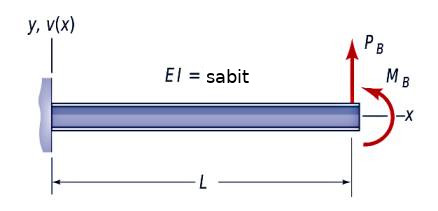
\includegraphics[width=15em]{phy_020_strs_05_03.jpg}

Sol ucu sabit bir dirsekli kiriş (cantilevel beam) var. Bu kirişe dikey yönde en
sağ ucunde $P_B$ yükü ve $M_B$ momenti uygulanıyor. Bu sistemde eğim $v'(x)$ ve
sapma $v(x)$ için gereken ifadeyi bulalım.

Uygulanan iki kuvvet kirişi yukarı doğru eğer, o zaman eğim alttakine benzer,

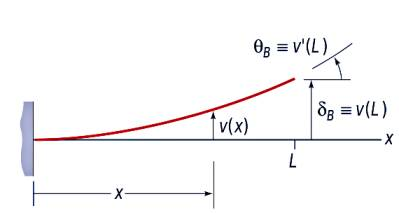
\includegraphics[width=15em]{phy_020_strs_05_04.jpg}

$M(x)$ bulmak için herhangi bir noktadaki hissedilen momentlerin toplamının
sıfır olduğunu hatırlayalım,

$$
M(x) - P_B(L-x) - M_B = 0
$$

Moment-eğri denklemini (3) kullanalım, ve üsttekileri o denkleme koyalım,

$$
EIv'' = M(x) = P_B(L-x) - M_B
$$

Aradığımız sonuç $v$ ve $v'$. O zaman üstteki denklemi iki kere entegre etmemiz
gerekli.

$$
EI v' = M_B x + P_B Lx - P_B \left( \frac{x}{2} \right)^2 + C_1
\mlabel{4}
$$

$$
EIv = M_B \left( \frac{x^2}{2} \right) +
P_B L  \left( \frac{x^2}{2} \right) -
P_B \left( \frac{x^3}{6} \right) +
C_1 x + C_2
\mlabel{5}
$$

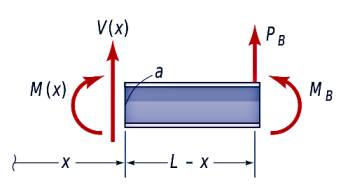
\includegraphics[width=15em]{phy_020_strs_05_05.jpg}

Şimdi sınır şartlarını probleme uygulayalım, bu değerler bilinenler
olarak bilinmeyen değerlerin bulunmasına yardımcı olacak. Sınır şartları
problem tanımında tarif edildi, kirişin bir ucu sabitlenmiş o zaman
$x=0$ noktasında hem eğim hem de sapma sıfır olmalı. Yani

$$
v'(0) = 0,\quad v(0) = 0
$$

Şartlardan ilkini $v'(0)=0$ ve $x=0$ kullanırsak (4) şu hale gelir,

$$
EI v' = C_1 = 0
$$

$v(0)=0$ ve $x=0$ kullanırsak (5) şöyle olur,

$$
EIv = C_2 = 0
$$

Demek ki (4) ve (5) şöyle yazılabilir,

$$
v'(x) = \frac{1}{EI} \left[
  M_B x + P_B Lx - P_B \left( \frac{x}{2} \right)^2
\right]
$$

$$
v(x) = \frac{1}{EI} \left[
  M_B \left( \frac{x^2}{2} \right) + 
  P_B L  \left( \frac{x^2}{2} \right) -
  P_B \left( \frac{x^3}{6} \right)
\right]
$$

Artık üstteki formülleri kullanarak kirişin en son noktasında, yani $x=L$'de, ya
da $B$ yerinde, sapmanın ne olacağını hesaplayabiliriz. Yerine koyarsak, sapma
$\delta_B$ diyelim,

$$
\delta_B = v(L) =
\frac{1}{EI} \left[
M_B \left( \frac{L^2}{2}  \right) +
P_B \left( \frac{L^3}{3}  \right)
\right]
$$


Aynı noktadaki sapma açısı $\theta_B$

$$
\theta_B = v'(L) =
\frac{1}{EI} \left[
M_B L + P_B \left( \frac{L^2}{2} \right) 
\right]
$$

Bir diğer formda denklemler şöyle gösterilebilir,

$$
\delta = \left( \frac{L^3}{3EI} \right) P +
\left( \frac{L^2}{2EI} \right) M
$$

$$
\theta = \left( \frac{L^2}{2EI} \right) P +
\left( \frac{L}{EI} \right) M
$$

Ustteki formulleri $P,M$ esitlikleri olarak tekrar duzenleyebiliriz.
Birinci formulu $\frac{3EI}{L^3}$ ikincisini $\frac{2EI}{L^2}$ ile
carparsak mesela her iki formulde $P$ tek basina kalir, ikinci formulden
birinciyi cikartip $P$'ler iptal edilir, basitlestirme sonrasi $M$ elde
edilir, benzer sekilde $P$ bulunur, sonuc

$$
P = \left( \frac{12EI}{L^3}  \right) \delta -
\left(  \frac{6EI}{L^2} \right) \theta
$$

$$
M = - \left( \frac{6 EI}{L^2}  \right) \delta +
\left( \frac{4 EI}{L}  \right) \theta
$$

Kaynaklar

[1] Bayramlı, {\em Fizik, Materyel Mekaniği - Hazırlık}

[2] Craig, {\em Mechanics of Materials, Third Edition}

[3] Bayramlı, {\em Çok Değişkenli Calculus, Eğrilik (Curvature)

\end{document}
